\section{Mini-Task 1: Parametric Analysis of a Microstrip Line}
\label{sec:minitask1}

The goal of this mini-task is to analyze how different parameters affect the characteristic 
impedance $Z_0$ of a microstrip line, using the \textit{LineCalc} tool in Keysight ADS software.

\subsection{A. Effect of Frequency on $Z_0$}

The frequency is swept from 5~GHz to 20~GHz in steps of 1~GHz, with $W$ and $L$ kept fixed.

\begin{figure}[h]
    \centering
    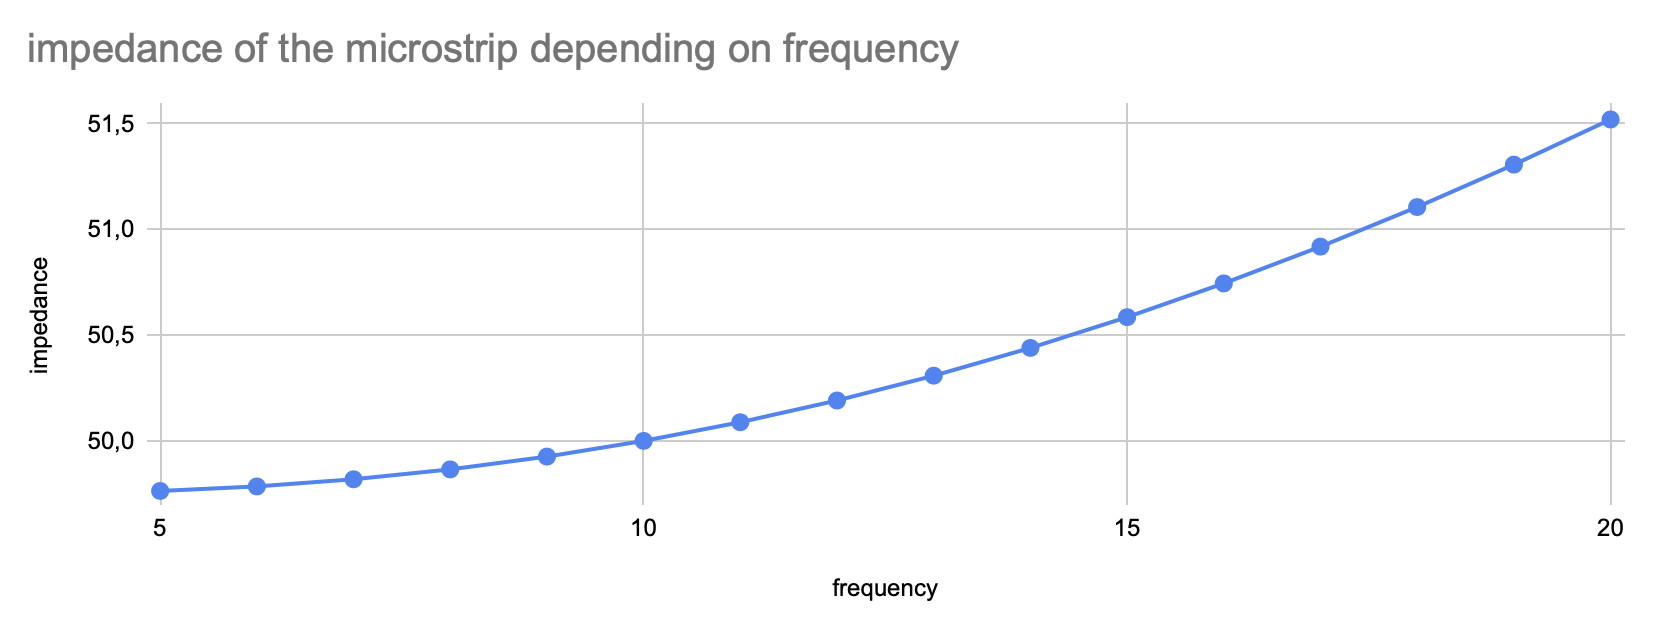
\includegraphics[width=\linewidth]{images/minitask1_impedance_vs_frequency.png}
    \caption{$Z_0$ versus frequency (5--20~GHz).}
    \label{fig:zo_freq}
\end{figure}

The results show that $Z_0$ increases steadily with frequency: from 49.76~$\Omega$ at 5~GHz 
up to 51.52~$\Omega$ at 20~GHz, which is a total change of about 1.76~$\Omega$ over the whole 
range. The reference value of 50~$\Omega$ is found exactly at 10~GHz, which matches the design 
target. The change is small and fairly linear, which means that frequency has a \textbf{limited 
effect} on $Z_0$ around the working frequency for this configuration.

\subsection{B. Effect of Substrate Parameters on $Z_0$}

\subsubsection{Relative Permittivity $\varepsilon_r$}

$\varepsilon_r$ is varied from 6.9 to 12.9 in steps of 1, with all other parameters kept at 
their reference values.

\begin{figure}[h]
    \centering
    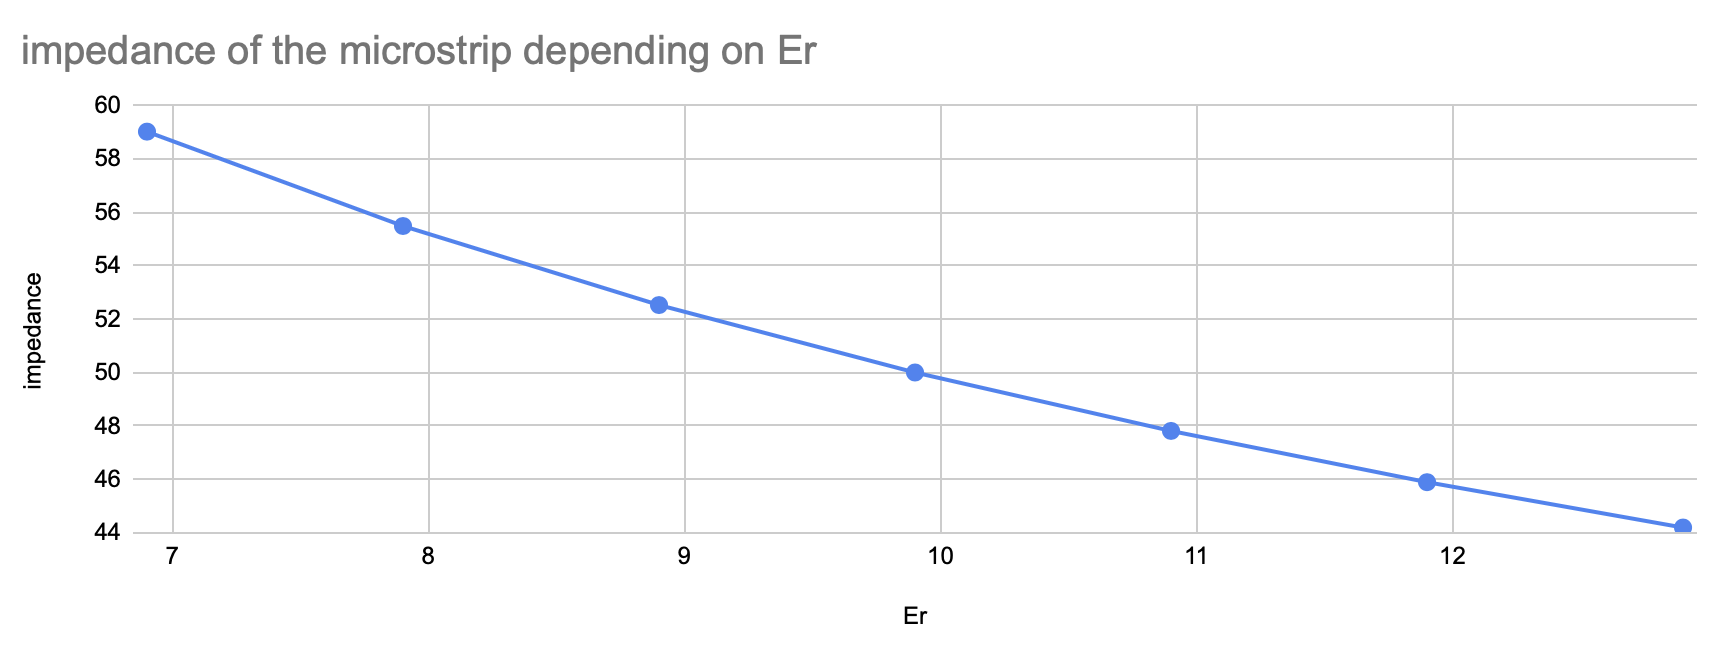
\includegraphics[width=\linewidth]{images/minitask1_impedance_vs_permittivity.png}
    \caption{$Z_0$ versus $\varepsilon_r$.}
    \label{fig:zo_er}
\end{figure}

The results show a clear \textbf{decreasing} relationship between $\varepsilon_r$ and $Z_0$: 
from 59.01~$\Omega$ at $\varepsilon_r = 6{.}9$ down to 44.20~$\Omega$ at $\varepsilon_r = 12{.}9$, 
which is a change of about 15~$\Omega$. The reference value of 50~$\Omega$ is recovered at 
$\varepsilon_r = 9{.}9$, as expected. A substrate with a higher permittivity stores more electric 
energy, which increases the capacitance per unit length of the line and therefore reduces $Z_0$. 
The relative permittivity is therefore a \textbf{significant} parameter for the characteristic 
impedance.

\subsubsection{Loss Tangent $\tan\delta$}

$\tan\delta$ is varied from 0.01 to 0.05 in steps of 0.01.

\begin{figure}[h]
    \centering
    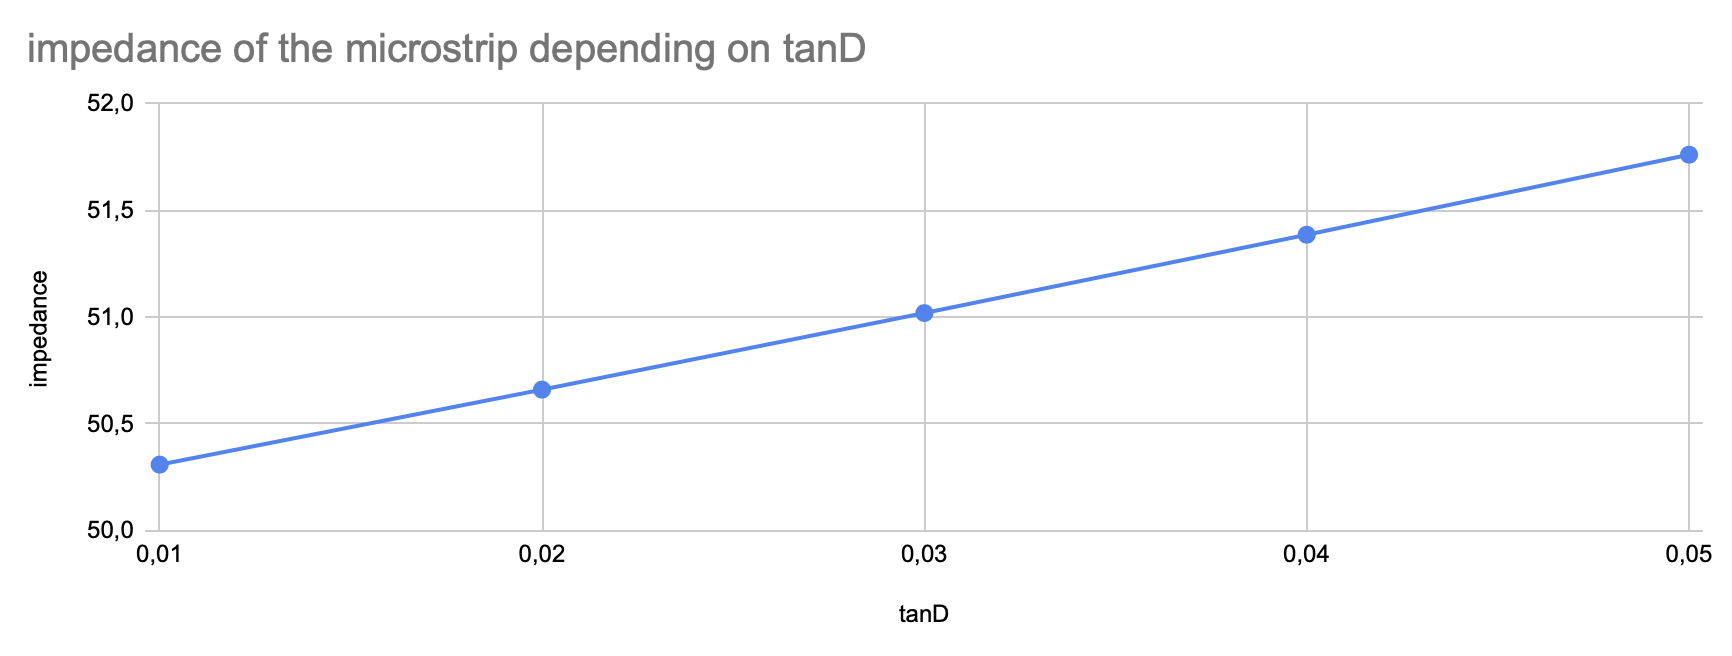
\includegraphics[width=\linewidth]{images/minitask1_impedance_vs_tanD.png}
    \caption{$Z_0$ versus $\tan\delta$.}
    \label{fig:zo_tand}
\end{figure}

$Z_0$ goes from 50.31~$\Omega$ at $\tan\delta = 0{.}01$ up to 51.76~$\Omega$ at 
$\tan\delta = 0{.}05$, which is a change of only about 1.45~$\Omega$ over the whole tested range. 
This is very small, which confirms that $\tan\delta$ has a \textbf{negligible effect} on $Z_0$. 
This parameter describes how lossy the substrate is and mainly affects how much the signal is 
attenuated along the line, not the impedance itself.

\subsubsection{Substrate Thickness $H$}

$H$ is varied from 0.1~mm to 1~mm in steps of 0.1~mm.

\begin{figure}[h]
    \centering
    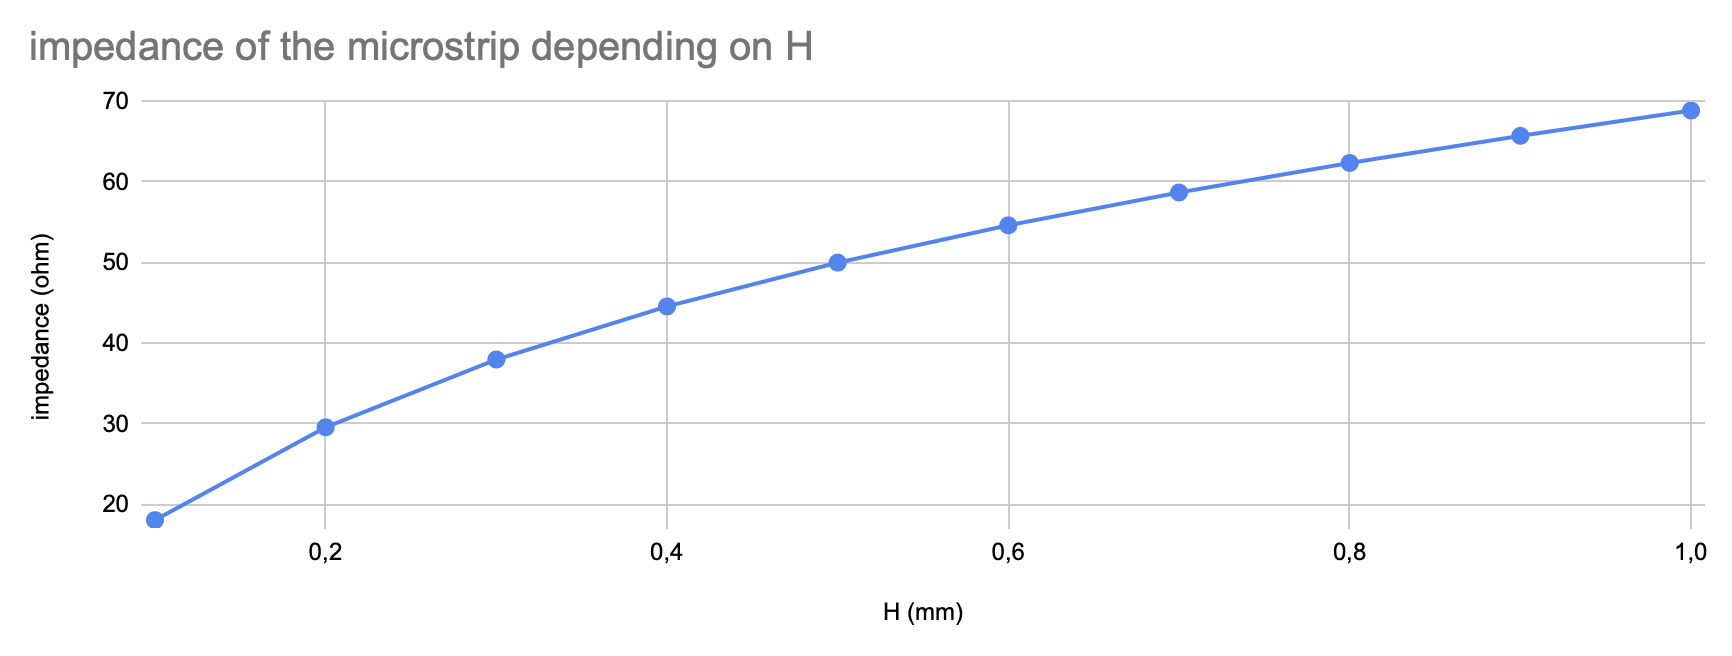
\includegraphics[width=\linewidth]{images/minitask1_impedance_vs_H.png}
    \caption{$Z_0$ versus substrate thickness $H$.}
    \label{fig:zo_H}
\end{figure}

This is the largest variation observed among the substrate parameters: $Z_0$ goes from 
18.08~$\Omega$ at $H = 0{.}1$~mm up to 68.86~$\Omega$ at $H = 1$~mm, a total change of 
about 50~$\Omega$. The relationship is \textbf{increasing and non-linear}: $Z_0$ changes 
quickly for small values of $H$ and then more slowly as $H$ gets larger. The reference value 
of 50~$\Omega$ is found at $H = 0{.}5$~mm. When the substrate is thicker, the top conductor 
is further from the ground plane, which reduces the capacitive coupling between the two and 
increases $Z_0$. The substrate thickness $H$ is the \textbf{most influential} substrate 
parameter on $Z_0$ in the tested range.

\subsection{C. Effect of the Line's Physical Parameters on $Z_0$}

\subsubsection{Conductor Width $W$}

$W$ is varied from 0.1~mm to 1~mm in steps of 0.1~mm.

\begin{figure}[h]
    \centering
    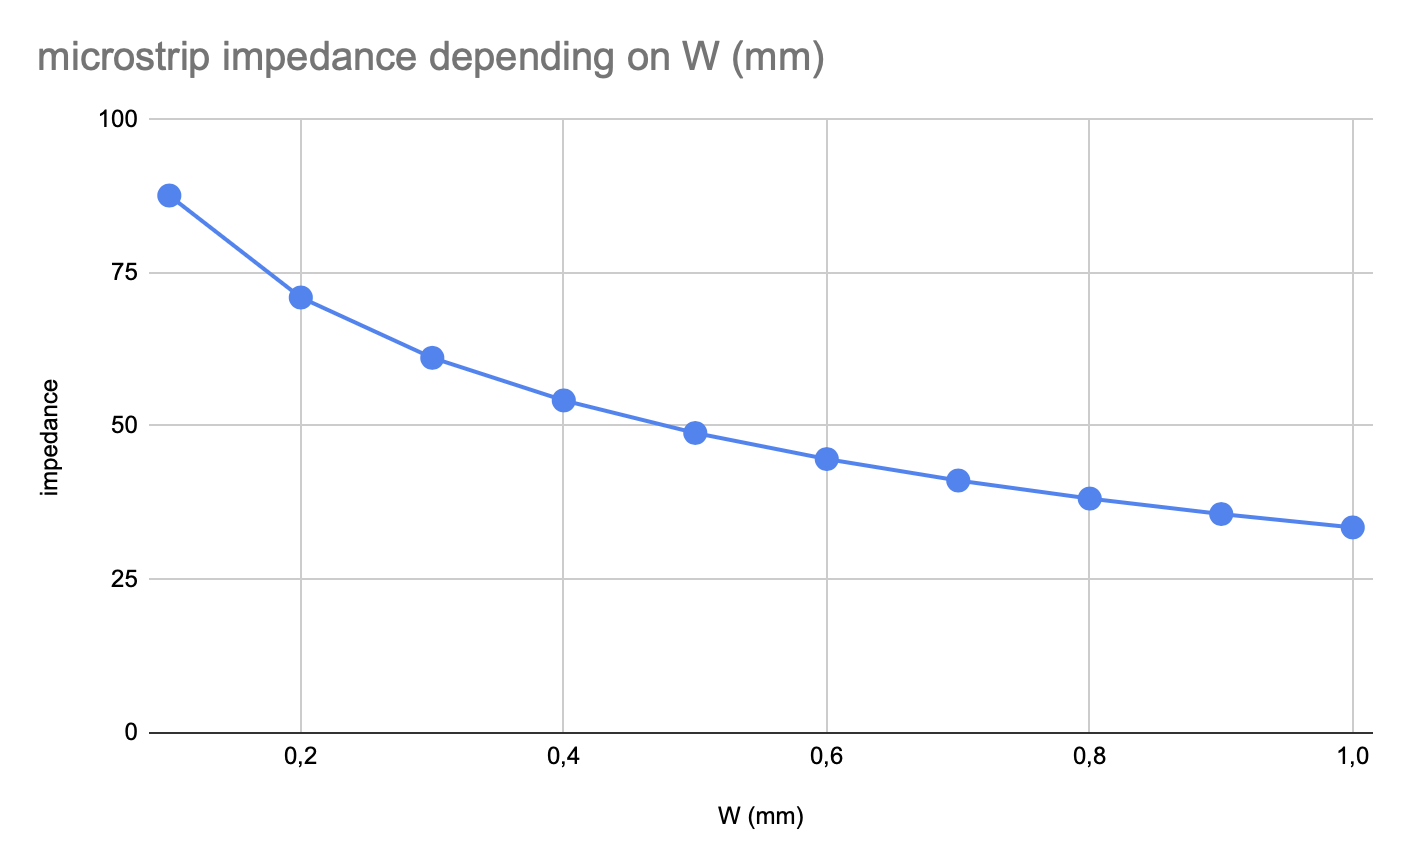
\includegraphics[width=\linewidth]{images/minitask1_impedance_vs_W.png}
    \caption{$Z_0$ versus conductor width $W$.}
    \label{fig:zo_W}
\end{figure}

$Z_0$ drops strongly as $W$ increases: from 87.54~$\Omega$ at $W = 0{.}1$~mm down to 
33.39~$\Omega$ at $W = 1$~mm, a total change of about 54~$\Omega$. The relationship is 
\textbf{decreasing and non-linear}: $Z_0$ drops fast for small widths, then more slowly 
as $W$ gets larger. A wider conductor increases the capacitance per unit length while 
reducing the inductance per unit length, which lowers $Z_0$. The width $W$ is therefore 
the physical parameter that \textbf{mainly controls} the characteristic impedance of 
the line.

\subsubsection{Line Length $L$}

$L$ is varied from 10~mm to 100~mm in steps of 10~mm.

\begin{figure}[h]
    \centering
    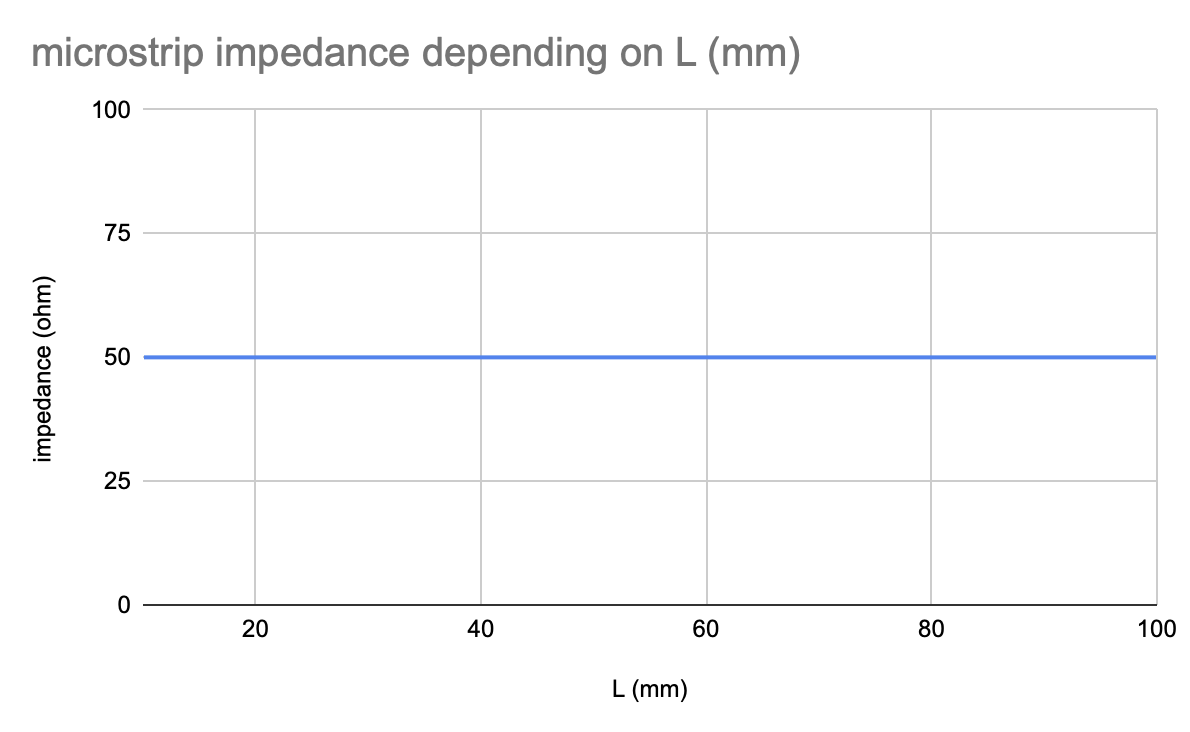
\includegraphics[width=\linewidth]{images/minitask1_impedance_vs_L.png}
    \caption{$Z_0$ versus line length $L$.}
    \label{fig:zo_L}
\end{figure}

$Z_0$ stays \textbf{perfectly constant} at 50~$\Omega$ for every value of $L$ tested. 
This is an important result: the characteristic impedance only depends on the cross-section 
of the line, meaning its geometry ($W$, $H$) and the substrate properties ($\varepsilon_r$). 
The length $L$ only affects the phase shift introduced by the line (electrical length 
$E_\text{eff}$), but has \textbf{no effect} on $Z_0$.

\subsection{Conclusion of Mini-Task 1}

\begin{table}[h]
\centering
\begin{tabular}{lcc}
\hline
\textbf{Parameter} & \textbf{$Z_0$ range obtained} & \textbf{Effect on $Z_0$} \\
\hline
Frequency (5--20~GHz)      & 49.76 -- 51.52~$\Omega$ & Small        \\
$\varepsilon_r$ (6.9--12.9)& 44.20 -- 59.01~$\Omega$ & Significant  \\
$\tan\delta$ (0.01--0.05)  & 50.31 -- 51.76~$\Omega$ & Negligible   \\
$H$ (0.1--1~mm)            & 18.08 -- 68.86~$\Omega$ & Dominant     \\
$W$ (0.1--1~mm)            & 33.39 -- 87.54~$\Omega$ & Dominant     \\
$L$ (10--100~mm)           & 50~$\Omega$ (constant)  & None         \\
\hline
\end{tabular}
\caption{Summary of the effect of each parameter on $Z_0$.}
\label{tab:synthese_minitask1}
\end{table}

This analysis clearly shows that the parameters with the most influence on $Z_0$ are the 
substrate thickness $H$ and the conductor width $W$, both causing a change of around 
50~$\Omega$. The relative permittivity $\varepsilon_r$ has a moderate but significant 
effect (~15~$\Omega$), while frequency and $\tan\delta$ have very little impact. The line 
length $L$ has no effect at all on $Z_0$, which confirms the basic definition of the 
characteristic impedance of a transmission line.